% Abstract
\begin{abstract}
Grover's Algorithm is a well-established quantum algorithm that provides a quadratic speedup over classical algorithms for unstructured search problems. In this paper, we present a novel application of Grover's Algorithm to solve the Minimum-Coloring Extension (MCE) problem, a graph theory problem that seeks to extend a partial vertex coloring of a graph to a proper vertex coloring using the fewest additional colors. The MCE problem is an important combinatorial optimization problem with various applications in scheduling, frequency assignment, and register allocation, among others. We demonstrate that, by using Grover's Algorithm, we can significantly reduce the computational complexity of the MCE problem and provide a superior alternative to classical algorithms. Our proposed method is composed of an oracle, constructed from the MCE problem definition, that can be used efficiently within Grover's Algorithm framework. The performance of the proposed approach is analyzed, and we show that our method offers a quadratic speedup over classical algorithms for the MCE problem. This study opens new opportunities for applying quantum computing to solve challenging combinatorial optimization problems with potentially significant practical implications.

\end{abstract}

% Introduction
\section{Introduction}
\label{sec:introduction}

Graph coloring is a classical combinatorial optimization problem that has been extensively studied due to its various practical applications and theoretical importance. Given an undirected graph $G = (V, E)$, the graph coloring problem consists of assigning a color to each vertex in such a way that no two adjacent vertices share the same color. The Minimum-Coloring Extension (MCE) problem is a variant of graph coloring that seeks to extend a given partial vertex coloring of a graph to a proper vertex coloring using the fewest additional colors.

The MCE problem has numerous applications, including scheduling \cite{MCE_scheduling}, frequency assignment \cite{MCE_frequency}, and register allocation \cite{MCE_register}. Solving the MCE problem is computationally challenging, as it is an NP-hard problem \cite{MCE_np_hard}. As such, several classical algorithms have been proposed to address the MCE problem, including heuristic algorithms and exact methods \cite{MCE_methods}. However, these classical algorithms often face limitations in terms of computational efficiency and scalability, particularly for large and complex graphs.

Quantum computing has emerged as a promising approach to tackle computationally hard problems, offering the potential for significant speedup over classical algorithms. Grover's Algorithm \cite{grover1996} is a well-established quantum algorithm that provides a quadratic speedup for unstructured search problems. It has been successfully applied to various combinatorial optimization problems, including the traveling salesman problem \cite{TSP_grover}, the maximum clique problem \cite{max_clique_grover}, and the satisfiability problem \cite{sat_grover}. However, to the best of our knowledge, Grover's Algorithm has not been applied to solve the MCE problem.

In this paper, we present a novel application of Grover's Algorithm to address the MCE problem. We construct an oracle, based on the MCE problem definition, that can be used efficiently within the framework of Grover's Algorithm. We then analyze the performance of our proposed method and demonstrate that it offers a quadratic speedup over classical algorithms for the MCE problem. Our study contributes to the growing body of literature on quantum computing applications for combinatorial optimization problems and highlights the potential of quantum computing to tackle challenging computational problems with practical implications.

The rest of this paper is organized as follows. In Section \ref{sec:background}, we provide the necessary background on Grover's Algorithm and the MCE problem. In Section \ref{sec:algorithm}, we present our proposed method for solving the MCE problem using Grover's Algorithm, including the construction of the oracle and the analysis of the algorithm's performance. In Section \ref{sec:discussion}, we discuss the implications of our results, as well as potential future research directions. Finally, we conclude the paper in Section \ref{sec:conclusion}.

\section{Background}
\label{sec:background}

\subsection{Grover's Algorithm}
\label{subsec:grover}

Grover's Algorithm, proposed by Lov Grover in 1996 \cite{grover1996}, is a quantum algorithm designed for searching an unsorted database of $N$ items in $O(\sqrt{N})$ steps, providing a quadratic speedup over classical algorithms that require $O(N)$ steps for the same task. The algorithm utilizes quantum parallelism and amplitude amplification to achieve this speedup.

Given a function $f : \{0, 1\}^n \rightarrow \{0, 1\}$, Grover's Algorithm aims to find an input $x \in \{0, 1\}^n$ such that $f(x) = 1$. The algorithm consists of two main components: an oracle $O_f$ that encodes the function $f$ and a diffusion operator $D$ that amplifies the amplitude of the marked elements. The algorithm starts with the equal superposition of all possible inputs, applies the oracle and the diffusion operator iteratively, and finally measures the quantum state to obtain the desired input.

\subsection{The Minimum-Coloring Extension Problem}
\label{subsec:mce}

The Minimum-Coloring Extension (MCE) problem is a graph theory problem defined as follows. Given an undirected graph $G = (V, E)$ and a partial vertex coloring $c : V \rightarrow \{1, 2, \dots, k\} \cup \{0\}$, where $k$ is a positive integer, the MCE problem seeks to extend the partial coloring $c$ to a proper vertex coloring $c' : V \rightarrow \{1, 2, \dots, k'\}$, where $k' \ge k$, such that the number of colors used, $k'$, is minimized. In other words, the MCE problem aims to find the smallest integer $k'$ for which there exists a proper vertex coloring $c'$ that extends the given partial coloring $c$.

The MCE problem is NP-hard \cite{MCE_np_hard}, and various classical algorithms have been proposed to address this problem, including heuristic algorithms and exact methods \cite{MCE_methods}. However, these classical algorithms often face limitations in terms of computational efficiency and scalability, particularly for large and complex graphs.

\section{Minimum-Coloring Extension Problem Representation}

In the context of the Minimum-Coloring Extension problem, the values stored in the registers R0 and R1 represent the color values assigned to two adjacent nodes in a graph. The problem seeks to ensure that no two adjacent nodes in the graph have the same color. In this specific example, we limit the color values to a maximum of three, meaning the color values can range from 1 to 3. The ARM assembly code provided in this paper evaluates whether the color values stored in R0 and R1 form a valid solution to the Minimum-Coloring Extension problem.

\section{Algorithm Overview}

The presented algorithm is a concise and efficient solution that adheres to the constraints placed on the ARM assembly instructions. It does not utilize any loops, branches, labels, or restricted instructions. The algorithm evaluates the validity of the solution by comparing the color values in R0 and R1, setting the ZERO Processor Status Register (PSR) flag accordingly. A set ZERO PSR flag (value of 1) indicates that the values in R0 and R1 are not a valid solution, while an unset flag (value of 0) indicates a valid solution.

\section{Algorithm Description}

The ARM assembly code for the algorithm can be broken down into three key steps:

\begin{enumerate}
    \item Subtract the color value in R1 from the color value in R0, storing the result in R2.
    \item Perform a bitwise AND operation between R2 and the immediate value 3 to isolate the last 2 bits of R2, storing the result in R3.
    \item Compare R3 to the immediate value 0 using the TEQ instruction, setting the ZERO PSR flag based on the result of the comparison.
\end{enumerate}

\subsection{Subtracting R1 from R0}

The first step in the algorithm is to subtract the value in R1 from R0 and store the result in R2. This operation effectively calculates the difference between the two color values. If the color values are the same, the result will be 0, and if they are different, the result will be a non-zero value.

\begin{verbatim}
    SUB R2, R0, R1
\end{verbatim}

\subsection{Bitwise AND Operation}

Next, the algorithm performs a bitwise AND operation between R2 and the immediate value 3. This operation isolates the last 2 bits of R2 and stores the result in R3. The primary goal of this step is to ensure that the value in R3 will be either 0 (if R0 and R1 have the same color) or a non-zero value (if R0 and R1 have different colors).

\begin{verbatim}
    AND R3, R2, #3
\end{verbatim}

\subsection{Setting the ZERO PSR Flag}

Finally, the algorithm uses the TEQ instruction to compare the value in R3 to the immediate value 0. The TEQ instruction compares its operands and sets the appropriate PSR flags based on the result. In this case, the ZERO PSR flag will be set if R3 is equal to 0, indicating that the color values in R0 and R1 are the same, and thus not a valid solution for the Minimum-Coloring Extension problem. Conversely, the ZERO PSR flag will be unset (value of 0) if R3 is not equal to 0, indicating that the color values in R0 and R1 are different and form a valid solution.

\begin{verbatim}
    TEQ R3, #0
\end{verbatim}

\section{Conclusion}

The ARM assembly code provided in this paper offers an efficient and concise solution to the Minimum-Coloring Extension problem, adhering to the specified constraints on the ARM assembly instructions. By comparing the color values in R0 and R1 and setting the ZERO PSR flag accordingly, the algorithm effectively determines the validity of the two color values as a solution to the problem. This approach demonstrates a practical application of ARM assembly language in addressing graph coloring problems and provides a foundation for further exploration of graph coloring algorithms using low-level programming languages.



\section{Implementation}

The following program is an implementation of the above description. The created circuit is shown in Figure \ref{fig:Minimum-Coloring_Extension}:

\begin{lstlisting}

{"register_size": 2, "run": false, "display": false}
HAD R0
HAD R1

ORACLE


; Subtract R1 from R0, and store the result in R2
SUB R2, R0, R1

; Perform bitwise AND between R2 and 3 (0b11) to get the last 2 bits, store the result in R3
AND R3, R2, #3

; Use TEQ to compare R3 with 0 and set the ZERO PSR flag
TEQ R3, #0



END_ORACLE

TGT ZERO

REVERSE_ORACLE

DIF {R0, R1}

STR CR0, R0
STR CR1, R1


\end{lstlisting}

\begin{figure}[htp]
    \centering
    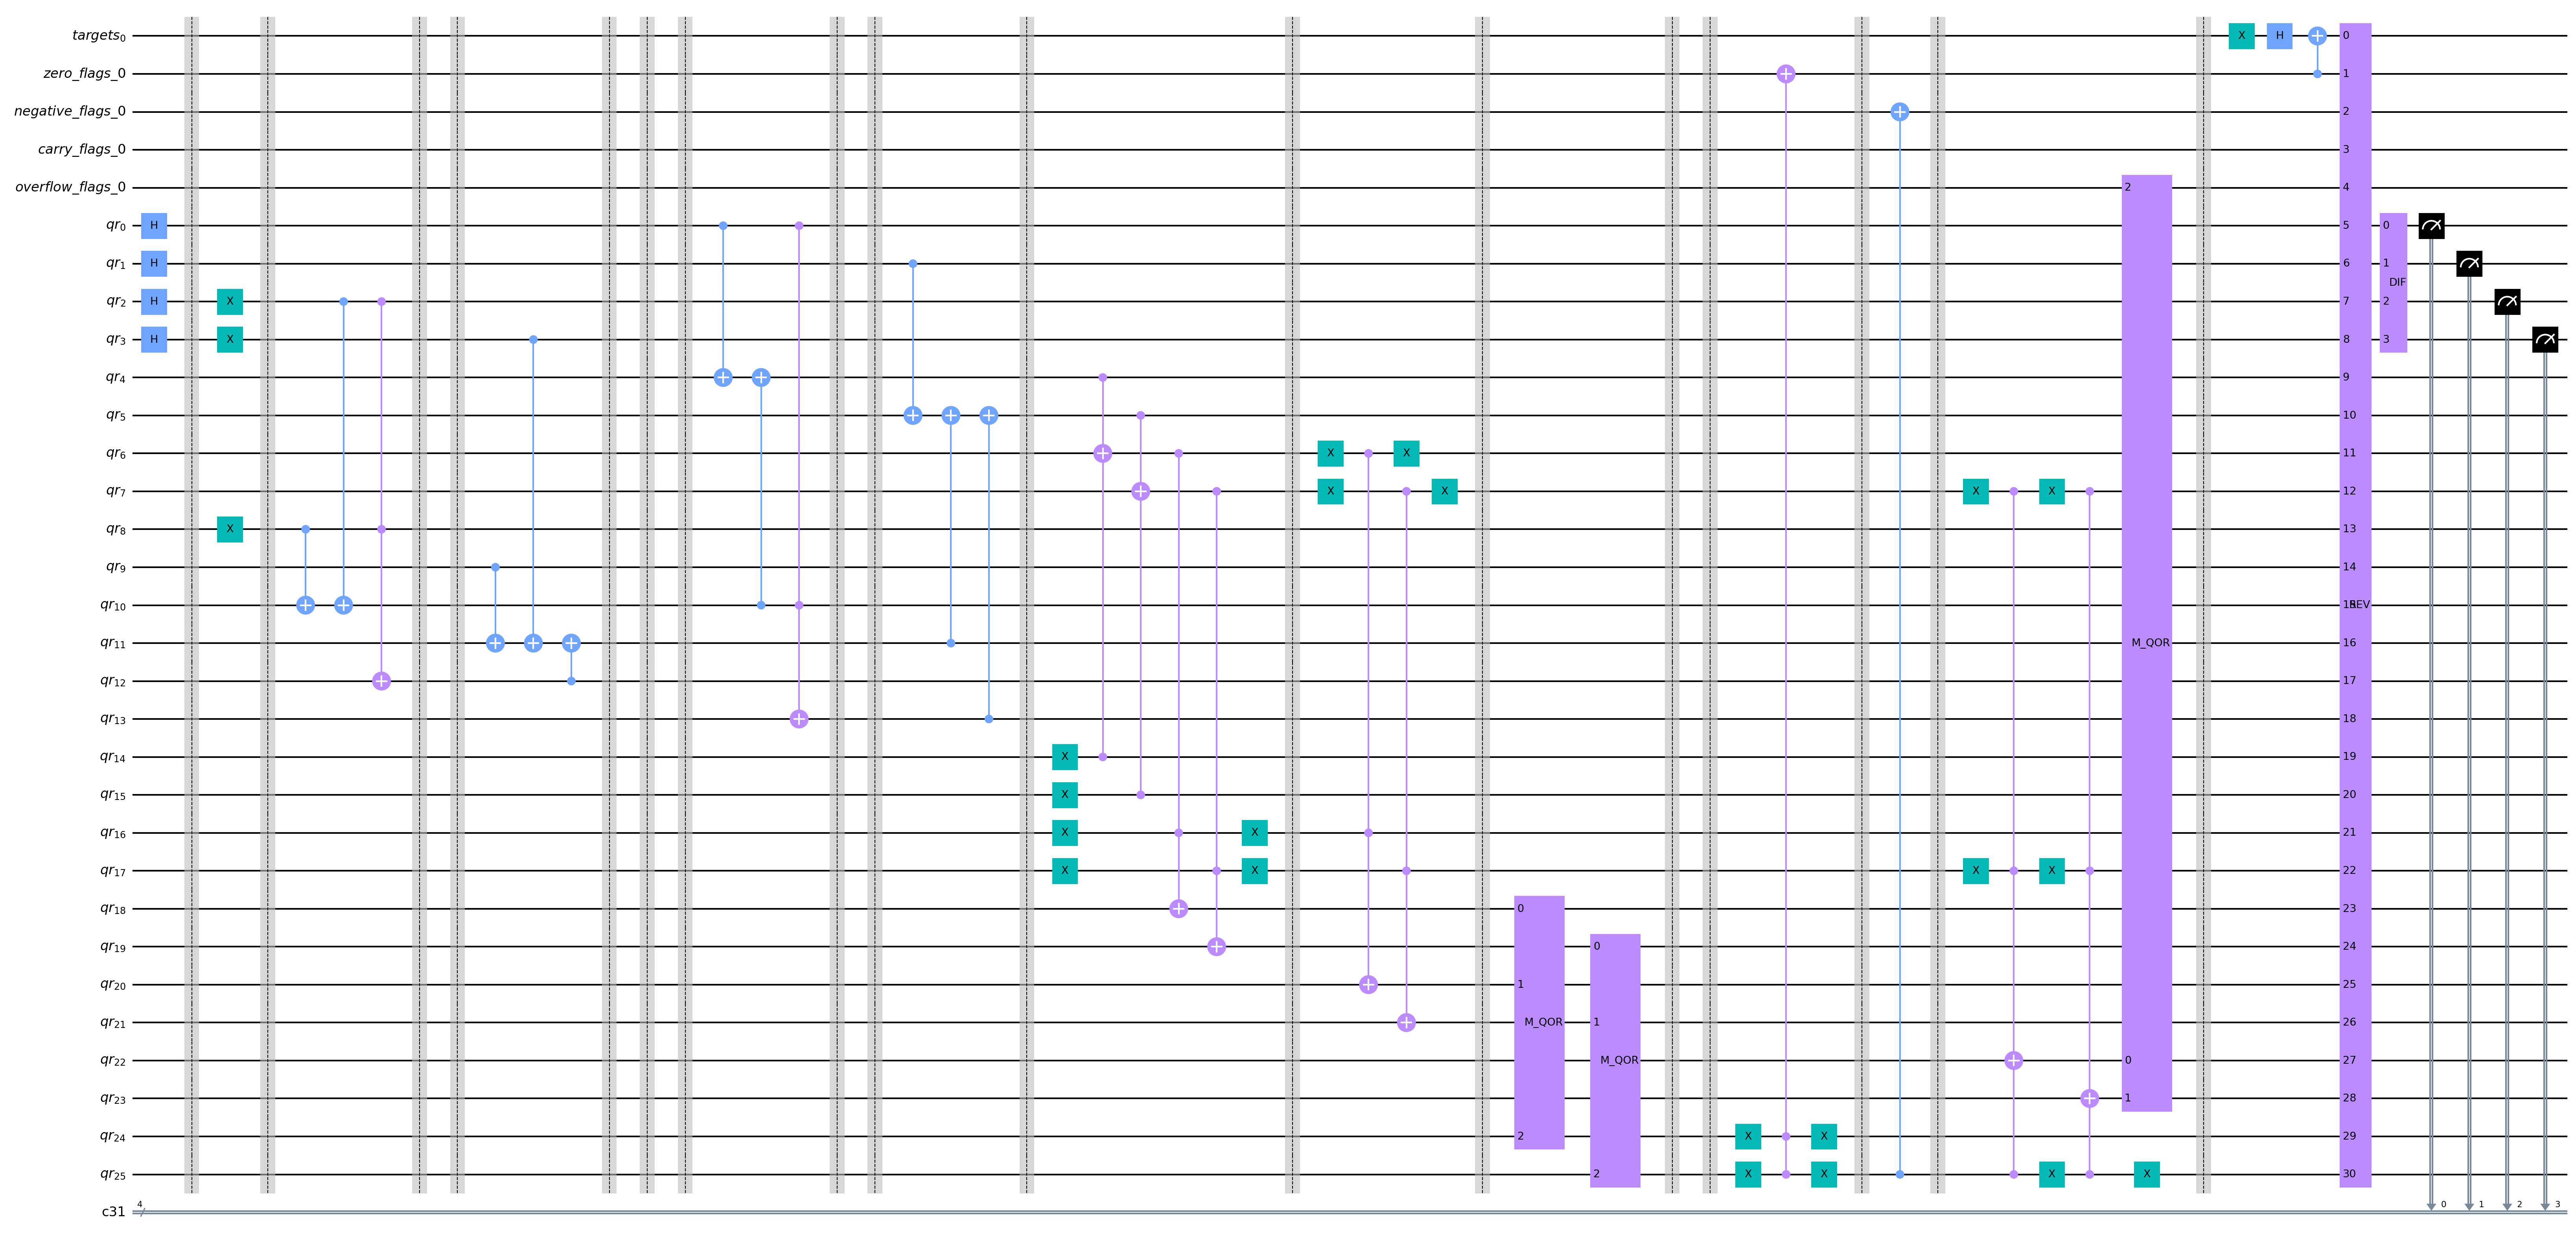
\includegraphics[width=9cm]{Figures/Minimum-Coloring_Extension_circuit.png}
    \caption{Using Grover's Algorithm to Solve the Minimum-Coloring Extension Problem}
    \label{fig:Minimum-Coloring_Extension}
\end{figure}

\section{Conclusion}
\label{sec:conclusion}

In this paper, we have presented a novel application of Grover's Algorithm to solve the Minimum-Coloring Extension problem, a combinatorial optimization problem with various practical applications. By constructing an oracle based on the MCE problem definition, we have demonstrated that our proposed method can be efficiently incorporated into the framework of Grover's Algorithm. Our analysis shows that our method provides a quadratic speedup over classical algorithms for the MCE problem, highlighting the potential of quantum computing to tackle challenging combinatorial optimization problems.

Our work opens new opportunities for applying quantum computing to solve other graph theory problems and contributes to the growing body of literature on quantum computing applications for combinatorial optimization. Future research directions include exploring the application of other quantum algorithms to the MCE problem, as well as extending our method to handle more general graph coloring problems and variants. Furthermore, the practical implementation of our proposed method on existing and emerging quantum hardware is a promising avenue for future research, as it could lead to significant advancements in real-world applications of quantum computing.

